%lezione 11 del 1 aprile 2026
%-----------------------------------------------------------------------------------------------------
\subsection{Esempio: l'effetto Bohm-Aharonov}
\begin{multicols}{2}
\begin{figure}[H]
    \centering
    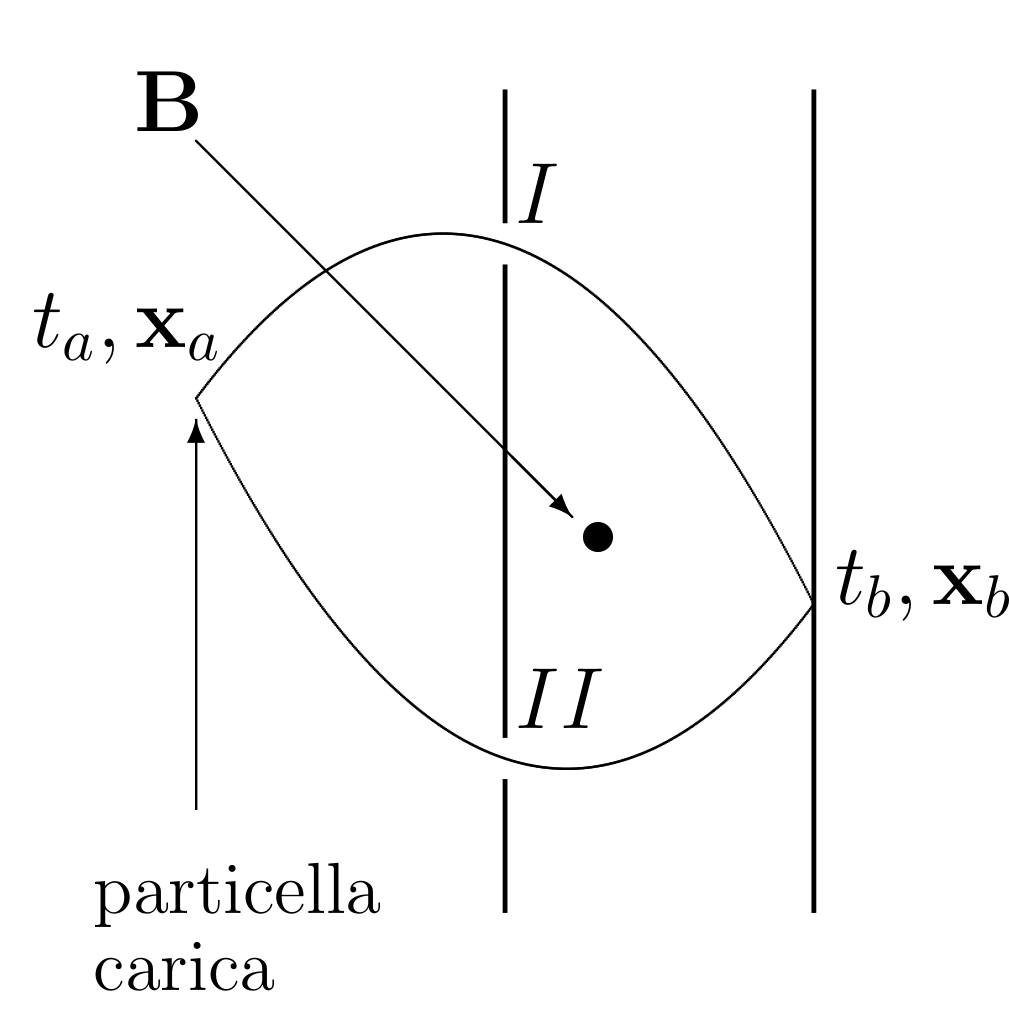
\includegraphics[width = .7\linewidth]{./bohm_a.png}
    \caption{\small Setup sperimentale}
    \label{fig:bohm}
\end{figure}
Un interessante esempio di problema facilmente risolubile con i \textit{path integral} è una variazione
del famoso esperimento delle due fenditure: si costringe una particella carica a passare
attraverso due fenditure macroscopicamente distanti e, come è noto, si osserva su uno schermo la figura
di interferenza.\\
Si consideri ora un campo magnetico localizzato tra le fenditure, di modo che il suo
effetto sia praticamente nullo nella zona dei cammini classici della particella, come in figura
\ref{fig:bohm}: si osserva sperimentalmente che la figura di interferenza cambia al variare del
campo magnetico $B$.
\end{multicols}
Vista la distanza tra le fenditure, anche nel limite semiclassico il campo non "tocca" la funzione
d'onda della particella, ma l'evidenza sperimentale afferma diversamente.

Per comprendere il motivo di questo effetto non locale del campo magnetico è necessario fare un po'
di conti.\\
Si consideri, come in figura, una particella di carica $q$ che parte dal punto $x_a\in\mathbb{R}^3$
al tempo $t_a$ e raggiunge il punto $x_b$ al tempo $t_b$: per semplicità si pone
$$\psi(x_a,t_a) = \delta^3(x-x_a) \rightarrow K(x_b,t_b,x_a,t_a) = \psi(x_b,t_b)$$
Il campo magnetico $B$ è costante, quindi si sceglie il gauge $\varphi=0$, $A(x,t)=A(x)$ e la
lagrangiana del sistema è
$$L(x,\dot x,A) = \frac{1}{2}m\dot x^2 + \frac{q}{c}\mathbf{\dot x}\cdot \mathbf{A} = L_0+L_B$$
dove $L_0$ è la lagrangiana della particella libera.

L'azione corrispondente è (ponendo $\frac{q}{c}=1$)
$$S = S_0 + \frac{q}{c}\int_{t_a}^{t_b}\mathbf{\dot x}\cdot \mathbf{A} = S_0+\int_{\gamma}d\mathbf{x}
\cdot \mathbf{A}$$

A differenza della trattazione precedente, in questo caso ci sono due cammini classici possibili:
il propagatore totale, nell'approssimazione semiclassica, è la somma del propagatore relativo al 
cammino $\gamma_I$ e di quello relativo al cammino $\gamma_{II}$:
$$K(x_b,t_b,x_a,t_a) = K_I + K_{II}$$
L'approssimazione semiclassica implica che 
$$K_i = e^{\frac{i}{\hbar}S_{cl,i}}\int_{}^{}\mathcal{D}\omega\exp\left\{\frac{i}{\hbar}S_{2,i}[\omega]
\right\}$$
con $i=I,II$

Poiché $L_B$ dipende linearmente da $\mathbf{\dot x}$, essa contribuisce solo in $S_{cl,i}$ e non
alle perturbazioni di ordine $\geq2$ in $S_{2,i}$: il propagatore per il cammino $\gamma_i$ vale dunque
$$K_i = \exp\left\{\frac{i}{\hbar}\int_{\gamma_i}d\mathbf{x}\cdot\mathbf{A}\right\}K_{0,i}$$
dove $K_{0,i}$ è il propagatore della particella libera sul cammino $\gamma_i$.\\
Si trova dunque che il propagatore per questo sistema fisico è
$$K(x_b,t_b,x_a,t_a) = \psi(x_b,t_b) =
\exp\left\{\frac{i}{\hbar}\int_{\gamma_I}d\mathbf{x}\cdot\mathbf{A}\right\}\psi_{0,I}(x_b,t_b) +
\exp\left\{\frac{i}{\hbar}\int_{\gamma_{II}}d\mathbf{x}\cdot\mathbf{A}\right\}\psi_{0,II}(x_b,t_b)$$
raccogliendo una fase globale $\theta=\frac{1}{\hbar}\int_{\gamma_I}^{}d\mathbf{x}\cdot\mathbf{A}$,
si trova che
$$\psi(x_b,t_b) = e^{i\theta}\left(\psi_{0,I}(x_b,t_b) +
\exp\left\{\frac{i}{\hbar}\oint_{\gamma_{II}-\gamma_I} d\mathbf{x}\cdot\mathbf{A}\right\}
\psi_{0,II}(x_b,t_b)\right)$$
e si riconosce immediatamente la circuitazione di \textbf{A} che, per il teorema di Stokes, è pari 
al flusso del campo magnetico $\Phi_B$ attraverso la superficie con bordo $\gamma_{II}-\gamma_I$.\\
Reinserendo $\frac{q}{c}$, si trova infine che
$$\boxed{\psi(x_b,t_b)=e^{i\frac{q}{c}\theta}\left(\psi_{0,I}(x_b,t_b)+\exp\left\{\frac{iq}{\hbar c}
\Phi_B\right\}\psi_{0,II}(x_b,t_b)\right)}$$
La variazione della figura di interferenza è dunque da attribuirsi al flusso di \textbf{B} che produce
un effetto non locale.

\textbf{Oss.} È qui evidente che la quantità \textit{non} gauge-invariante \textbf{A} contribuisce solo
con una (trascurabile) fase globale, mentre ciò che produce effetti osservabili è il flusso di
\textbf{B}, che è gauge-invariante.

\textbf{Oss.} I valori per cui il campo magnetico non cambia la figura di interferenza sono quelli tali
che $\frac{q}{\hbar c}\Phi_B = 2n\pi \leftrightarrow \Phi_B = n\frac{2\pi\hbar c}{q}$, cioè i multipli
interi del magnetone di Bohr $\mu_B$.

